\documentclass[tikz,border=8pt]{standalone}
\usepackage{amsmath,amssymb}
\usetikzlibrary{arrows.meta,automata,positioning,quotes}
\begin{document}
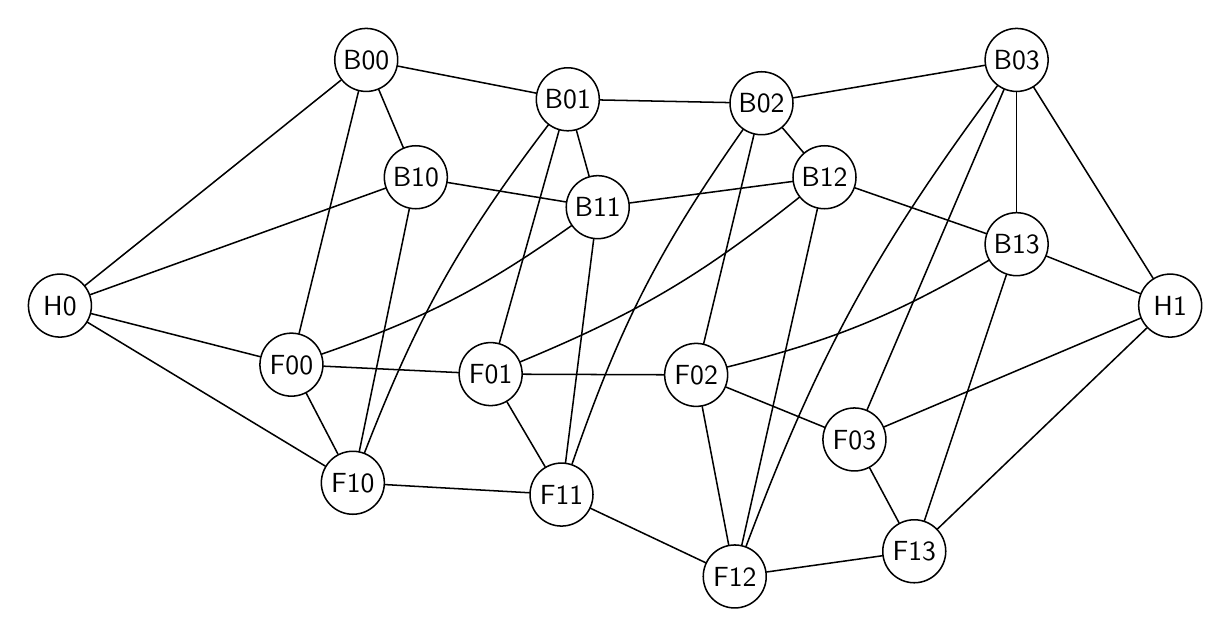
\begin{tikzpicture}[x=1cm,y=1cm]
\tikzset{
  graphnode/.style={circle,draw=black,line width=0.55pt,minimum size=8mm,inner sep=1pt,font=\sffamily},
  graphedge/.style={draw=black,line width=0.55pt,line cap=round,line join=round},
  directed/.style={graphedge,-{Stealth[length=2.4mm,width=2.0mm]}},
  undirected/.style={graphedge}
}
\node[graphnode] (n_F00) at (-1.16,-0.15) {F00};
\node[graphnode] (n_F01) at (1.37,-0.27) {F01};
\node[graphnode] (n_F02) at (3.98,-0.28) {F02};
\node[graphnode] (n_F03) at (5.99,-1.10) {F03};
\node[graphnode] (n_F10) at (-0.38,-1.65) {F10};
\node[graphnode] (n_F11) at (2.27,-1.80) {F11};
\node[graphnode] (n_F12) at (4.47,-2.84) {F12};
\node[graphnode] (n_F13) at (6.75,-2.52) {F13};
\node[graphnode] (n_B00) at (-0.21,3.72) {B00};
\node[graphnode] (n_B01) at (2.35,3.22) {B01};
\node[graphnode] (n_B02) at (4.81,3.17) {B02};
\node[graphnode] (n_B03) at (8.05,3.72) {B03};
\node[graphnode] (n_B10) at (0.42,2.23) {B10};
\node[graphnode] (n_B11) at (2.73,1.85) {B11};
\node[graphnode] (n_B12) at (5.61,2.23) {B12};
\node[graphnode] (n_B13) at (8.05,1.38) {B13};
\node[graphnode] (n_H0) at (-4.10,0.60) {H0};
\node[graphnode] (n_H1) at (10.00,0.60) {H1};
\draw[undirected] (n_F00) -- (n_F01);
\draw[undirected] (n_F01) -- (n_F02);
\draw[undirected] (n_F02) -- (n_F03);
\draw[undirected] (n_F10) -- (n_F11);
\draw[undirected] (n_F11) -- (n_F12);
\draw[undirected] (n_F12) -- (n_F13);
\draw[undirected] (n_F00) -- (n_F10);
\draw[undirected] (n_F01) -- (n_F11);
\draw[undirected] (n_F02) -- (n_F12);
\draw[undirected] (n_F03) -- (n_F13);
\draw[undirected] (n_B00) -- (n_B01);
\draw[undirected] (n_B01) -- (n_B02);
\draw[undirected] (n_B02) -- (n_B03);
\draw[undirected] (n_B10) -- (n_B11);
\draw[undirected] (n_B11) -- (n_B12);
\draw[undirected] (n_B12) -- (n_B13);
\draw[undirected] (n_B00) -- (n_B10);
\draw[undirected] (n_B01) -- (n_B11);
\draw[undirected] (n_B02) -- (n_B12);
\draw[undirected] (n_B03) -- (n_B13);
\draw[undirected] (n_F00) -- (n_B00);
\draw[undirected] (n_F01) -- (n_B01);
\draw[undirected] (n_F02) -- (n_B02);
\draw[undirected] (n_F03) -- (n_B03);
\draw[undirected] (n_F10) -- (n_B10);
\draw[undirected] (n_F11) -- (n_B11);
\draw[undirected] (n_F12) -- (n_B12);
\draw[undirected] (n_F13) -- (n_B13);
\draw[undirected] (n_F00) to[bend right=8] (n_B11);
\draw[undirected] (n_F01) to[bend right=8] (n_B12);
\draw[undirected] (n_F02) to[bend right=8] (n_B13);
\draw[undirected] (n_F10) to[bend left=8] (n_B01);
\draw[undirected] (n_F11) to[bend left=8] (n_B02);
\draw[undirected] (n_F12) to[bend left=8] (n_B03);
\draw[undirected] (n_H0) -- (n_F00);
\draw[undirected] (n_H0) -- (n_F10);
\draw[undirected] (n_H0) -- (n_B00);
\draw[undirected] (n_H0) -- (n_B10);
\draw[undirected] (n_H1) -- (n_F03);
\draw[undirected] (n_H1) -- (n_F13);
\draw[undirected] (n_H1) -- (n_B03);
\draw[undirected] (n_H1) -- (n_B13);
\end{tikzpicture}
\end{document}
